\documentclass[a4paper]{article}

% The preceding line is only needed to identify funding in the first footnote. If that is unneeded, please comment it out.
\usepackage{cite}
\usepackage{amsmath,amssymb,amsfonts}
\usepackage{algorithmic}
\usepackage{graphicx}
\usepackage{textcomp}
\usepackage{xcolor}
\usepackage{pifont}
\usepackage[utf8]{vietnam}
\usepackage{subcaption}
\usepackage{setspace}
\usepackage{tabularx,booktabs}
\usepackage{relsize}
\usepackage{multicol}
\usepackage{etoolbox}%
\usepackage{xpatch}
\usepackage{blindtext}
\usepackage[a4paper,margin=1in,footskip=0.25in]{geometry}
\usepackage{indentfirst}
\usepackage{rotating}
\usepackage{placeins}

\setlength{\parindent}{1.5cm}
\setlength{\parskip}{0.5em}
% defined centered version of "X" column type:
\newcolumntype{C}{>{\centering\arraybackslash}X} 
\def\BibTeX{{\rm B\kern-.05em{\sc i\kern-.025em b}\kern-.08em
		T\kern-.1667em\lower.7ex\hbox{E}\kern-.125emX}}
\begin{document}
	
\section{Introduction}
In video understanding tasks, action recognition and detection are prominent and
meaningful due to their practical applications in daily life. Some notable
applications include Surveillance and Security, Human-Computer Interaction,
Sports Analysis, Entertainment and Gaming, among others. Although deep learning
models designed to solve these problems often require significant computational
resources, with the advancement of computer hardware, the deployment in
real-world scenarios while meeting real-time processing speed has become more
feasible over time.

Besides the requirement for significant computational resources, they also
demand a large and sufficiently complex dataset. In addition to serving as
training data, datasets also provide a portion of data specifically for
evaluating models, thereby establishing a common benchmark for comparing
different models. Over the years, new datasets have emerged, either as additions
to existing datasets or as entirely new ones based on different construction
perspectives. This has increased both the diversity and quantity of available
data, but also inadvertently posed challenges in selecting an appropriate
dataset. Evaluating whether a dataset is suitable for a given research problem
is not merely a matter of its scale. Other characteristics must also be
considered, such as the dataset creator's perspective, data collection methods,
sample size, number of classes, level of annotation detail (spatial, temporal,
sound, etc.), popularity within the research community, the baseline for
comparison, and various other factors. Therefore, it is necessary to carefully
examine datasets relevant to the task, gather information, evaluate, and then
compare them to ultimately select the desired dataset for research purposes.
This process typically consumes a significant amount of time and effort. To
address this issue, in this paper, we aim to compile notable datasets in the
fields of action detection and action recognition, listing them chronologically
while providing concise necessary information regarding:

\begin{itemize}
	\item \textit{Context and construction perspective of the dataset}: Since the
	datasets are presented chronologically, this section clarifies the information
	regarding the background and the authors' perspectives on the shortcomings or
	the necessary additions to older datasets.
	\item \textit{Dataset distribution}: Information about the dataset, such as the
	number of data samples, the number of classes, the train-validation splits, and
	any other available details.
	\item \textit{Annotations}: Explanation of the annotations provided in the
	dataset.
	\item \textit{Data collection methods}: We summarize the data collection
	process employed by the respective author groups on that dataset. This allows
	for a more objective assessment of the dataset's reliability and quality based
	on the researcher's perspective.
\end{itemize}

In section II, we will provide a brief overview of the history and context of
the field of artificial intelligence research from its inception to the
emergence of CNN models and their dominance from image task to video task.
Having a general understanding of the history and context will help readers
understand why datasets have their limitations and continue to evolve over the
years.

In section III, we list the datasets in the order of their publication time
(measured from the time the accompanying paper is published). Each dataset
includes four sections presented in the following order: "Context
and Construction Perspective of the Dataset," "Annotations," "Dataset
Distribution," and "Data Collection Methods." If some information is not
provided by the authors in the original paper, it will be left blank or omitted.
Additionally, if the authors provide any additional information included in the
dataset, we will allocate a separate section below to describe it. The list of
datasets, along with a brief overview of their publication dates and the
mentioned data quantities, can be found in Fig1..
\section{Overview History}
Although the field of artificial intelligence emerged in the mid-1990s, it took
several decades for significant progress to be made, thanks to the remarkable
advancements in computer hardware - greater computing power and easier
accessibility. As a result, the research community's interest in AI has
significantly increased. AI competitions began to be organized, particularly in
computer vision, attracting numerous research groups. In 2010, the ImageNet
Large Scale Visual Recognition Challenge (ILSVRC) \cite{ILSVRC} was initiated,
aiming to build upon the success of the PASCAL VOC challenge \cite{PASCALVOC} by
evaluating model performance in image recognition tasks.

ILSVRC, upon its initial launch, garnered significant attention and credibility
within the research community due to its unprecedented scale of data: 1.2
million training images and 1,000 object classes. It attracted participation
from top researchers in the field and further solidified its reputation.

\begin{figure} [h]
	\centering
	
	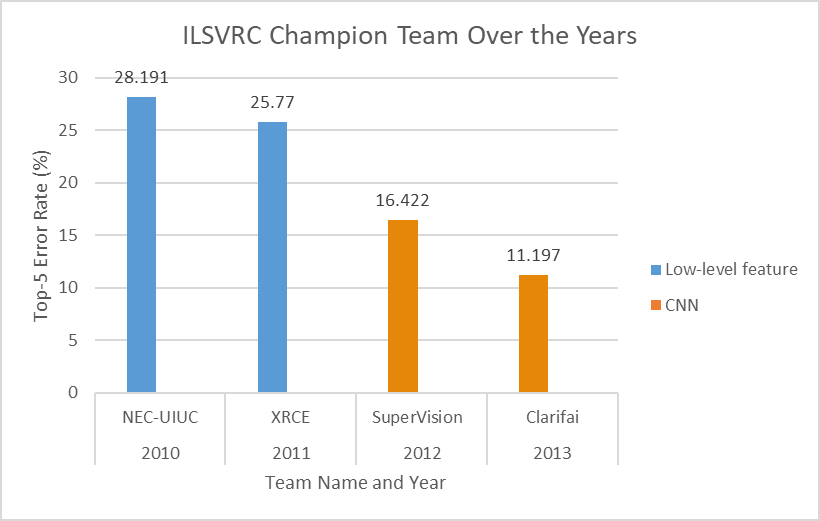
\includegraphics[width=1.\linewidth]{fig_info/fig1/ILSVRCChampionTeamOvertheYears}
	\caption{ILSVRC champion team over years on classification task}
	\label{fig:ilsvrcchampionteamovertheyears}
\end{figure}

Go back to 1998 when LeNet \cite{LeNet}, the first CNN model, was introduced. At
that time, CNN was just one of many research directions and had not received
much attention. It wasn't until 2012 when the SuperVison team, led by
researchers at the University of Toronto, proposed a CNN model called AlexNet
and convincingly won the ILSVRC2012 in image classification with a top-5 error
rate of only 16.422\% (Fig \ref{fig:ilsvrcchampionteamovertheyears}). They
completely outperformed other competitors at that time, paving the way for the
era of CNN and the dawn of Deep Learning. Since then, winning solutions in
subsequent years of ILSVRC have consistently utilized CNN. Over time, there has
been an increasing number of research studies applying CNN models to various
tasks. Through experimentation, CNN has proven to be effective not only in image
classification but also in localization, segmentation, and even beyond computer
vision, extending to other fields such as speech processing and natural language
processing. CNN has shown great potential in developing solutions for previously
challenging problems that were not adequately addressed. One such problem is
action recognition, which is a highly significant task with practical
applications. CNN has opened up possibilities for developing solutions to
previously unresolved problems, and action recognition is just one of them,
receiving considerable attention and practical implications.

The problem of Action Recognition existed before the rise of CNN. Solutions for
action recognition during this period often involved feature extraction using
various methods to obtain a feature vector from the data, followed by a
classifier, typically a Support Vector Machine (SVM). This approach is called
"hand-crafted feature" and it continued to dominate other methods, including
CNNs, until 2015 because CNN models were still relatively new and not
extensively explored. Over time, the research community gradually replaced these
hand-crafted feature methods with CNNs. Continuous advancements and proposals of
CNN models for action recognition have been made, such as Two-stream networks,
Segment-based methods, Multi-stream networks, 3D CNNs, and so on. Alongside
these developments, there has been an increasing demand for computational power
and a significant growth in the amount of data. The datasets used in this period
were also limited, as shown in Table \ref{config}, which lists prominent
datasets from before 2012. It can be observed that in terms of scale (number of
classes, number of video clips), the datasets were still quite limited.

\begin{table}[h]
	\centering
	%\small
	\caption{Action recognition dataset}
	\begin{tabular}{l|l l l l}
		\toprule
		Name & Year & NumClass & Clip/Class & Ref \\
		\midrule
		KTH & 2004 & 6 & 100 & \cite{KTH} \\
		Weizmann & 2005 & 9 & 9 & \cite{Weizmann} \\
		IXMAS & 2007 & 11 & 33 & \cite{IXMAS} \\
		Hollywood & 2008 & 8 & 30-129 & \cite{HollyWood} \\
		UCF Sports & 2008 & 9 & 14-35 & \cite{UCFSports} \\
		Hollywood2 & 2009 & 12 & 61-278 & \cite{Hollywood2} \\
		UCF YouTube & 2009 & 11 & 100 & \cite{UCFYouTube} \\
		Olympic & 2010 & 16 & 50 & \cite{Olympic} \\
		\bottomrule
	\end{tabular}%
	\label{config}
\end{table}%

Building a dataset typically goes through four steps: (1) Defining a set of
predefined actions, (2) Collecting videos from data sources, (3) Annotating the
data (either automatically, semi-automatically, or manually), (4) Cleaning and
filtering the data to remove duplicates and noise. Each step presents its own
challenges. In step (1), defining an action is not a simple task as humans often
perform complex combinations of gestures. So, what constitutes an "atomic
action"? In step (2), do the video sources comply with copyright rules? Privacy
regulations? Is the dataset stable (not prone to loss or replacement)? In step
(3), the workload scales with the dataset size, and there can be vague
boundaries in determining the start and end of an action. In step (4), what
criteria are used to evaluate whether a video meets the standards for usability?
There are many related questions, such as the availability of human and
financial resources, required to meet the demands of building a comprehensive
research dataset. Furthermore, considering the context before CNNs gained
significant prominence, investing in developing a large-scale dataset was highly
risky.

CNN models possess immense power that scales with their complexity., is prone to
overfitting, especially when dealing with small amounts of data. During the
explosion of CNN, research groups faced many challenges due to data scarcity.
Methods like data augmentation were effective solutions, but it was still
necessary to supplement larger and more complex datasets to meet the growing
demand for data in CNN models. Another reason is that the remarkable success of
CNNs in image processing tasks has been greatly contributed by large-scale
datasets like ImageNet. However, in the video domain, there is currently no
comparable dataset to ImageNet. Realizing this need, research groups from all
over the AI research community have continuously improved and published
increasingly refined datasets. These datasets play a crucial role as a common
benchmark for comparing different models.
\section{Overview Dataset}
Nói về context và sơ lược về thông tin, quy mô của bộ dữ liệu.
\subsection{HMDB51}
In 2011, HMDB51 \cite{HMDB51} was introduced to highlight differences among action categories based on motion rather than static poses, which were commonly used in datasets like KTH \cite{KTH} and Weizmann \cite{Weizmann}. With the growing demand for datasets that present more substantial challenges and enhance the capabilities of action recognition systems, HMDB51 aims to enrich the contextual background and increase the number of action categories, thereby improving the utility of recognition systems in real-life applications.

It includes 6,766 video clips covering 51 different action categories sourced from movies and Internet, with each category having at least 101 clips. Each video contains a single action described in its name, with a quality of 240px and length of more than 1 second.
\subsection{UCF101}
Introduced in 2012 as an expansion of UCF50 by adding 51 classes, UCF101 \cite{UCF101} aimed to refine and expand the range of actions captured in the previous datasets, contributing to a more comprehensive understanding of human activities. Additionally, the dataset also blurs the difference between artificial and real-life videos, therefore accurately reflects the diversity of human actions represented in real-world scenarios. Among the four versions of the UCF family: "UCF Sports \cite{UCFSports}, UCF11 \cite{UCFYouTube}, UCF50, and UCF101", the dataset being referred to is the largest and most widely used.

The dataset contains 13,320 videos demonstrating 101 actions. Each clip has a resolution of 320x240 pixels at 25 FPS. Additionally, this dataset also includes audio data for 50 action classes. Each clip has its augmented version, which expands into various variants of itself, such as increasing or reducing the length, changing the segment, or adding audio.
\subsection{Sport-1M}
In 2014, Sport-1M \cite{Sports1M} was developed to apply CNN methods to action recognition categories, marking a departure from datasets such as HMDB51 \cite{HMDB51} and UCF101 \cite{UCF101}, which were designed to accommodate traditional machine learning methods, especially SVM, thus became non-equivalent. Therefore, with the rise of CNNs, there has been encouragement to develop equivalent resources that can enhance their capabilities.

The dataset contains 1,133,158 YouTube videos, covering a diverse range of content. There are 487 unique classes in the dataset, with each class ranging from 1000 to 3000 videos. Notably, each video may be assigned multiple labels, indicating that a single video could have more than one annotation, accounting for approximately 5\% of the dataset.
\subsection{ActivityNet}
First introduced in 2015, ActivityNet \cite{ActivityNet} offer a solution with a large-scale dataset that provides a high level of specificity for human daily life in a hierarchical structure. At that time, UCF101 \cite{UCF101} and THUMOS-14 \cite{THUMOS} already have their own category distributions, but they lack detailed organization and depth of levels, which limits the amount of information they provide. This hierarchical organization allows for a detailed understanding of the diverse range of behaviors captured in this dataset, especially in every day activities.

In the version 1.3 released in Mar 2016, ActivityNet contains 849 hours from 27,801 videos of indoor actions with a total of 68.8 hours that appear 200 human-centric activities. Most of the videos have lengths ranging from 5 to 10 minutes at 30 FPS have HD resolution quality (1280x720). 
\subsection{Youtube-8M}
In 2016, YouTube-8M \cite{YouTube8M} was introduced as the largest multi-label video classification dataset, which utilized the content-based annotation method. Unlike previous datasets such as Sports-1M \cite{Sports1M} and ActivityNet \cite{ActivityNet}, which only assigned a limited number of action categories, YouTube-8M employed Knowledge Graph entities to filter topics presented on YouTube and therefore broadening the scope to cover a wide range of activities. The purpose of this dataset is to understand the main actions in the video and summarize them into key topics.

In the newest update in May 2018, YouTube-8M underwent a cleanup process to ensure quality for both video resolution and annotation vocabulary. It removed the private, unfamous and sensitive contents for safety purpose. Currently, the dataset comprises over 6.1 million video IDs from 3,862 entities, grouped into 24 high-level topics. Each video is required to be between 120 and 500 seconds long and must contain at least one target vocabulary. The dataset allows for multi-label assignments, with each video typically having an average of 3.0 assigned classes.

\subsection{Charades}
Introduced in 2016, Charades \cite{Charades} is described as "Hollywood in Homes" when using a man-made dataset instead of downloading videos from YouTube. Using a similar method to the Something \cite{Some} dataset, a group of AMT workers was hired to employ the Hollywood filming method to create clips from diverse environments. Due to the noisy labels and background context from datasets sourced from the internet, such as HMDB51 \cite{HMDB51} and UCF101 \cite{UCF101}, Charades aims to create a high-quality and realistic dataset, particularly focusing on daily activities.

The dataset comprises of 9,848 videos with an average length of 30 seconds, which demonstrates 157 action classes and 46 object classes. Overall, there are 27,847 video descriptions and 66,500 temporally localized action contributed by 267 people.
\subsection{Something Something}
Introduced its first version in 2017, Something V1 \cite{SomethingV1} emphasizes detailed interactions between human actions and objects, aiming to provide fine-grained videos that reflect real-world aspects. The YouTube-sourced datasets, such as Sport-1M \cite{Sports1M} or YouTube-8M \cite{YouTube8M}, although notably large in size, still involve combining features extracted from frames, thus becoming a "set of images" classification task.

When an action is combined with various objects, it can potentially mislead the model since it diverges from its learned associations due to the lack of contextual understanding of how different actions correlate with each other of datasets. As an illustration, consider the action of "pointing" which can result in two scenarios: "Pointing a finger" (Harmless) or "Pointing a knife" (Dangerous). The main objective of Something Something dataset is to address this problem.

In the newer V2 version released in 2018, the number of videos has increased to 220,847 clips, which is twice the number in V1, while retaining the same set of labels totaling 174. Additionally, each clip has been upgraded to a quality of 240px. Each clip has an average length of 2-6 seconds performing a single action at 12 FPS. Overall, there are 318,572 annotations, which involve 30,408 unique objects.
\subsection{Multi-THUMOS}
Expanding upon the THUMOS \cite{THUMOS} dataset, Multi-THUMOS \cite{Multi-THUMOS} represents a substantial advancement in action recognition datasets, offering multi-action sequences over time. Addressing limitations observed in previous datasets like UCF101 \cite{UCF101} and HMDB51 \cite{HMDB51}, as well as its precursor THUMOS, Multi-THUMOS provides dense multilabel annotations of fined-grained actions for untrimmed video footage, therefore enhancing the accurately localizing in multi-action reasoning.

Overall, Multi-THUMOS contains a total of 30 hours from 413 videos, demonstrating 65 action classes and 38,690 annotations. Those classes are expanded from the original THUMOS and are arranged in a hierarchical relationship. Inside that, instance actions last on average 3.3 seconds, with the shortest action in this dataset (throw) lasting 66 milliseconds. Each video in Multi-THUMOS can contain up to 25 action labels, with a maximum of 9 actions per frame, significantly improved from 3 action labels, with a maximum of 2 actions per frame from THUMOS. 
\subsection{Kinetics}
In 2017, one of the most famous action classification datasets, Kinetics \cite{Kinetics-400}, was introduced. Its method combines elements from the previous HMDB51 \cite{HMDB51} and UCF101 \cite{UCF101}datasets and expands the number of action classes to 400. By collecting videos from YouTube, the dataset can capture various camera motions, angles, lighting conditions, etc., and therefore covering a broad range of human actions.

Later in 2018, an updated version, Kinetics-600 \cite{Kinetics-600}, was introduced. Kinetics-600 is a superset of Kinetics-400, retaining the original 368 classes and splitting 32 classes to provide clearer explanations. Additionally, a new filtering method was used to gather videos correlated to the action classes. Due to some validation sets from Kinetics-400 becoming part of the Kinetics-600 test set, it is recommended not to evaluate Kinetics-600 with a pre-trained Kinetics-400 model.

In the next year, Kinetics-700 \cite{Kinetics-700} was added, expanding by 30\% compared to Kinetics-600. Additional actions were sourced partly from EPIC-Kitchens and AVA datasets, and some were split from previous action classes for more fine-grained information. Because of serving as an expansion, it is recommended to train on Kinetics-600 and then evaluate on Kinetics-700 to ensure the unseen results.

In 2020, the final version Kinetics-700-2020 \cite{Kinetics-700-2020} was introduced. It keeps the same action classes as the 700 version but increase the dataset's quality. Geographical diversity are increased, rare actions were gathered from more videos, and duplicated videos were removed. These changes resulted in a more balanced dataset.

The Kinetics dataset contains 10 seconds short clips demonstrating the mentioned action. The table below shows the size of the three Kinetics version:
\begin{center}
	\begin{tabular}{| l | l | l | l |}
		\hline
		Dataset & Total videos & Action classes & Average clips per class \\ \hline
		Kinetics-400 & 306,245 & 400 & 683\\ \hline
		Kinetics-600 & 495,547 & 600 & 762\\ \hline
		Kinetics-700-2020 & 647,907 & 700 &  926\\ \hline
	\end{tabular}
\end{center}

\subsection{AVA}
Introduced in 2018, AVA's \cite{AVA} main goal is to overcome weaknesses of previous datasets like Sports-1M \cite{Sports1M}, YouTube-8M \cite{YouTube8M}, Something Something \cite{SomethingV1}, and Moments in Time \cite{MomentsinTime}, which focus on large-scale datasets and are often annotated automatically, leading to noisy annotations. Other datasets such as ActivityNet \cite{ActivityNet}, THUMOS \cite{THUMOS}, and Charades utilize a large number of videos containing multiple actions but only provide temporal annotations. Therefore, AVA provides realistic fine-grained recognition in a complex environment where actors perform a set of combined actions, aiming to enhance spatio-temporal action localization.

Currently, there are four different versions of AVA. The newest version, v2.2, consists of a total of 430 videos covering 80 classes extracted from movies. Each video contributes 15 minutes of footage sampled at a rate of 1Hz, which translates to one frame per second, resulting in 897 segments per 15 minutes.

\subsection{EPIC-KITCHENS}
Since its first introduction in 2018, EPIC-KITCHENS-100 \cite{EPIC-KITCHENS} now extends to provide a fully version of a large-scale egocentric dataset. Recently, ATM workers are being frequently utilized to collect desired video footage scripted scenarios, resulting in great contributions to projects like Something Something \cite{SomethingV1} and Hollywood in Home \cite{Charades}. However, this practice also leads to a lack of natural actions in real life. Given that situation, EPIC-KITCHENS captures random multitasking actions performed by real individuals without any scripts. By recording daily kitchen activities from the first-person perspective of 32 participants from 10 different countries, it aims to present a challenging real-life scenario.

The number of records in the dataset amounts to 55 hours in length. Within it, 39,596 action segments and 454,158 object bounding boxes are extracted. Recorded with GoPro devices, the clips are captured in Full HD resolution at 60 FPS, resulting in 11.5 million frames. The average length of each clip is 1.7 hours, starting from the moment the actor goes to their kitchen and ending when they finish their work, describing both the preparation and cooking process. After that, both objects and actions were annotated manually.

\subsection{Moments in Time}
In 2019, Moments in Time \cite{momentsintime} was introduced and became one of the largest datasets comprising hundreds of verbs depicting moments lasting a few seconds. Over the years, the rapid growth of datasets has expanded the usability of human action understanding. Large-scale video datasets such as Kinetics and YouTube-8M \cite{YouTube8M} play significant roles in studying open-world vocabulary from the internet. Other datasets, such as ActivityNet \cite{ActivityNet} and AVA \cite{AVA}, explore recognizing and localizing fine-grained actions by linking correlations. To enhance these characteristics, Moments in Time aims to ensure a high-quality and balanced dataset, capturing both inter- and intra-class variations across different levels of abstraction for video understanding.

The dataset contains more than 1,000,000 labeled 3-second videos, which include 339 action classes. The actors performing actions are not just limited to humans but also include animals or cartoon characters. Therefore, this dataset proposes a new challenge in recognizing events across various actors. Moreover, sound-dependent classes are added to expand the capability of understanding auditory cues.
\subsection{HACS}
HACS \cite{HACS} emerged in response to the increasing need for extensive datasets, facilitating the development of more sophisticated models in the realm of action recognition. Inspired by the notable expansions witnessed in large-scale action recognition datasets like Sport-1M, Kinetics, and Moments in Time, HACS enhances both its scale and quality to offer a more encompassing resource. Moreover, it builds upon the strengths of past action localization datasets such as THUMOS \cite{THUMOS}, AVA \cite{AVA}, Charades \cite{Charades}, and especially ActivityNet \cite{ActivityNet}. 

The dataset provides 504K videos sourced from YouTube, categorized into 200 action classes. These videos are trimmed into shorter segments, resulting in a total of 1.5M clips, each lasting 2 seconds, for more accurate labeling which is called HACS Segments. Then, it is annotated into positive (has action) and negative (doesn't has action) samples.
\subsection{HVU}
Introduced in 2020 as a multi-label and multi-task fully annotated dataset, HVU \cite{HVU} provides a multi-label and multi-task large-scale video benchmark with a comprehensive list of tasks and annotations for video analysis and understanding. CNNs model has envolved to be stronger and faster in recent years, but the datasets just allow them to recognize single label per task, which hinders the learning of ConvNets. 

HVU comprises a total of 572,000 videos and 3,143 labels. It consists of trimmed video clips with varying durations, capped at a maximum length of 10 seconds. Additionally, HVU does not solely rely on a single action class but instead includes multiple tags which is organized into six main categories: scene, object, action, event, attribute, and concept.
\subsection{AViD}
Introduced in 2020, AViD \cite{AViD} aims to provide an Anonymized Videos from Diverse Countries dataset. In the past, datasets such as Kinetics, HACS \cite{HACS}, and HVU \cite{HVU}, although containing numerous labeled video clips, were predominantly limited to the USA and other English-speaking countries. Moreover, those datasets were mainly sourced from YouTube links, which may not be available in some countries. AViD solves that problem by saving it as a static dataset, which can be found at the relevant link provided by the authors. When collecting videos, the authors blurred all the actors' faces to prevent machines from recognizing people in the videos but still reliably recognized actions, which is also a unique characteristic of this dataset.

After the filtering process, the dataset has a total of more than 800K videos from over the world, demonstrating 887 classes. The labels follow hierarchy structure from general to particular action for studying various aspects of action performance.
\subsection{FineAction}
Introduced in 2022, FineAction \cite{FineAction} aims to create a novel large-scale and fine-grained video dataset specialized in the temporal action localization task. Recently, many datasets have provided a diversity of temporal annotations such as ActivityNet \cite{ActivityNet}, Multi-THUMOS \cite{Multi-THUMOS}, and HACS \cite{HACS}; however, they lack detailed fine-grained annotations for daily activities. Hence, FineAction aims to address the weaknesses of those datasets and reduce annotation bias to ensure generalization. It also proposes a new challenge of fine-grained localization.
 
FineAction provides 16,732 untrimmed videos of 106 action categories, containing up to 103,324 temporal instances. The action classes are arranged in a three-level granularity of taxonomy hierarchy. At the top level, the dataset demonstrates coarse-grained actions, while at the bottom, it presents fine-grained ones. Each clip has an average duration of 7.1 seconds. Up to 11.5\% of the clips have multiple action labels with overlaps.
\subsection{Toyota Smarthome}
Toyota Smarthome \cite{ToyotaSmarthome} is introduced to provide a realistic daily action dataset captured by security cameras. Its purpose is to address the limitation of action generalization from UCF101 \cite{UCF101}, HMDB51 \cite{HMDB51}, and Kinetics \cite{Kinetics-400} when they can't demonstrate fine-grained daily living activities. Therefore, the dataset provides a diversity of both fine-grained and composite actions, performed by uninstructed actors.

The dataset consists of 31 daily living activities performed by 18 actors, resulting in 16,115 videos. The actions are acted randomly with no script provided, resulting in untrimmed videos for localization. Each action can have multiple camera views, ranging from 2 to 7. For action recognition, the number of video clips per activity spreads from the rarest action (cutting bread with 45 clips) to the most frequent action (walking with 4070 clips). Each action can have a variety of durations, from a few seconds (sitting down) to a few minutes (cleaning dishes).
\section{Analysis}
Các thông tin ở từng mục sẽ được nói kĩ nhưng không đi sâu vào từng bộ dữ liệu mà mang tính tổng quát, sau đó thống kê vào bảng. Thông tin trên bảng sẽ được điền dạng kí hiệu hoặc yes/no, sau đó chú thích bên dưới.

\subsection{Characteristic}
Based on the nature of each task provided in each dataset, we have divided the dataset into three main tasks: Localization, Detection, and Classification. Although the common classification approach only consists of two tasks, Detection and Recognition, we have found that defining three tasks as mentioned above makes it much easier to consolidate information.
 
\begin{itemize}
	\item \textbf{Localization}: This task requires our model to determine the time period during which an action occurs in a video. This can involve predicting the time of occurrence for the action in the video or providing predictions for each frame at the frame-level.

	\item \textbf{Detection}: The task of this is to identify which action (label) is being performed and where it is happening (bounding box) in each frame. This means our model needs to accurately identify the specific action taking place in the video and provide information about its location in each frame.

	\item \textbf{Classification}: The task involves determining the class (or multiple classes) of actions that the model believes are present in a given video. This requires our model to have the ability to classify and recognize different actions based on the content of the video.
\end{itemize}

\newcommand{\cmark}{\ding{51}}%
\newcommand{\xmark}{\ding{55}}%

Table \ref{characteristic} summarizes all the datasets analyzed in this paper. For some datasets such as ActivityNet \cite{ActivityNet} or YouTube8M \cite{YouTube8M}, which have later updated versions, we have also noted the version alongside the dataset name. However, the accompanying papers may not always be updated along with the dataset, so we cannot guarantee that the version mentioned in the paper will match the version stated in this paper. Nevertheless, the attached paper will at least be the initial version when the dataset was released. The datasets are arranged in chronological order of their release year. To provide a visual representation, the tasks associated with each dataset are marked with a \cmark, while the others are left blank. In order to be concise, except for the datasets mentioned above, the remaining information will not be reiterated in the tables in subsequent sections.

\begin{table}[h]
	\centering
	%\small
	\caption{Action recognition dataset}
	\renewcommand{\arraystretch}{1.5}
	\begin{tabular}{l|c|c|c c c}
		\toprule
		Name                    & Ref                       & Year & Localization & Detection & Classification\\
		\hline
		HMDB51                  & \cite{HMDB51}             & 2011 &              &           & \cmark         \\
		UCF101                  & \cite{UCF101}             & 2012 &              &           & \cmark         \\
		Sport-1M                & \cite{Sports1M}           & 2014 &              &           & \cmark         \\
		MultiTHUMOS             & \cite{Multi-THUMOS}       & 2015 & \cmark       &           &                \\
		ActivityNet(v1.3)       & \cite{ActivityNet}        & 2016 & \cmark       &           & \cmark         \\ 
		Charades                & \cite{Charades}           & 2016 & \cmark       &           & \cmark         \\
		Kinetics-400            & \cite{Kinetics-400}       & 2017 &              &           & \cmark         \\
		Kinetics-600            & \cite{Kinetics-600}       & 2018 &              &           & \cmark         \\
		Youtube-8M(v2018)       & \cite{YouTube8M}          & 2018 &              &           & \cmark         \\
		Something Something(v2) & \cite{SomethingSomething} & 2018 &              &           & \cmark         \\
		AVA(v2.2)               & \cite{AVA}                & 2018 &              & \cmark    &                \\
		Moments in Time(v1)     & \cite{MomentsinTime}      & 2018 &              &           & \cmark         \\
		HACS                    & \cite{HACS}               & 2019 & \cmark       &           & \cmark         \\
		Kinetics-700            & \cite{Kinetics-700}       & 2019 &              &           & \cmark         \\
		HVU                     & \cite{HVU}                & 2020 &              &           & \cmark         \\
		AViD                    & \cite{AViD}               & 2020 &              &           & \cmark         \\
		Kinetics-700-2020       & \cite{Kinetics-700-2020}  & 2020 &              &           & \cmark         \\
		Toyota Smarthome        & \cite{ToyotaSmarthome}    & 2020 & \cmark       &           & \cmark         \\
		EPIC-KITCHENS-100       & \cite{EPICKITCHENS100}    & 2021 & \cmark       &           & \cmark         \\	
		FineAction              & \cite{FineAction}         & 2021 & \cmark       &           &                \\
		\bottomrule
 		
	\end{tabular}%
	\label{characteristic}
\end{table}%

\subsection{Data construction method}

Each dataset has a different process for constructing the dataset, but in general, these processes share three main points: 1) Defining a list of action classes. 2) Data collection. 3) Annotation.
\begin{itemize}
	\item \textbf{Define action classes}: Typically, defining action classes is the first step in the aforementioned three-step process. Authors generally take two main approaches: relying on previous research or constructing action classes from scratch. However, there are also some datasets that define action classes during the annotation process.
	\begin{itemize}
		\item Based on previous research: (\textit{base one another research}) Datasets that rely on linguistic studies or utilize action classes from previous datasets (either fully or with additional modifications) fall into this category.
		
		\item Constructing action classes from scratch: (\textit{research}) Datasets that independently construct their own set of action classes without relying on any specific research (or with minimal reliance) are classified under this category.
	\end{itemize}
	
	\item \textbf{Collect video} : For datasets focusing on scale expansion, such as YouTube-8M \cite{YouTube8M}, they are often sourced from the internet (primarily from YouTube) due to the abundance of data. On the other hand, datasets focusing on fine-grained actions tend to utilize user-generated videos from crowdsources. This information is explicitly mentioned in the "Data Sources" column.
	
	\item \textbf{Annotation} : The annotation process can be classified into three main categories: manual, automatic, and hybrid.
	\begin{itemize}
		\item \textit{manually} : Manually labeling data typically involves hiring human labor from platforms like Amazon Mechanical Turk (AMT). Datasets that employ this method often have a small scale (e.g., HMDB51) or focus on fine-grained actions (e.g., Toyota Smart Home).
		
		\item \textit{automatically} : Using automatic labeling tools, these datasets often exhibit a high level of noise \cite{Sports1M}.
		
		\item \textit{hybrid} : Combining automatic and manual methods, typically involving the use of deep learning models for automated labeling followed by human verification, is often employed.
	\end{itemize}
	Additionally, there are \textit{predefined} labels, which means the data is searched based on existing labels and directly assigned to those labels.
\end{itemize}

Table \ref{DataCollectionMethod} summarizes the information mentioned above. Any unavailable information will be annotated as \textit{no mentioned}. Additionally, the annotation methods are also referenced in the Ann Protocol column.

\begin{sidewaystable}[h]
	\centering
	\caption{Action recognition dataset}
	\renewcommand{\arraystretch}{1.5}
	\begin{tabular}{l|c|c|c|c|c}
		\toprule  
		Name                    & ActList Construction Method     & Data Sources                    & Anno Method   & Ann Protocol  \\
		\hline
		HMDB51                  & research                 & Internet + digital movie        & manually      & No mentioned     \\
		UCF101                  & no mentioned             & YouTube                         & no mentiond   & No mentioned \\
		Sport-1M                & research                 & YouTube                         & automatically & No mentioned \\
		MultiTHUMOS             & base on another research & THUMOS                          & manually      & No mentioned \\
		ActivityNet(v1.3)       & base on another research & Online repositories             & hybrid        & AMT    \\ 
		Charades                & research                 & Crowdsourced record             & predefine     & AMT   \\
		Kinetics-400            & base on another research & YouTube                         & manually      & AMT\\
		Kinetics-600            & base on another research & YouTube                         & manually      & AMT\\
		Youtube-8M(v2018)       & research                 & YouTube                         & predefine     & No mentioned\\
		Something Something(v2) & research                 & Crowdsourced record             & predefine     & AMT\\
		AVA(v2.2)               & research                 & YouTube                         & hybrid        & Faster-RCNN, perembed, Hungarian\\
		Moments in Time(v1)     & base on another research & Youtube, Flickr, Vine etc       & hybrid        & AMT     \\
		HACS                    & base on another research & YouTube                         & hybrid        & Faster RCNN \\
		Kinetics-700            & base on another research & YouTube                         & manually      & AMT  \\
		HVU                     & research                 & YouTube-8M, Kinetics-600, HACS  & hybrid        & Google Vision API , Sensifai Video Tagging API \\
		AViD                    & base on another research & Flickr, Instagram etc           & hybrid        & AMT, I3D   \\
		Kinetics-700-2020       & base on another research & YouTube                         & manually      & AMT  \\
		Toyota Smarthome        & research                 & Crowdsourced record             & manually      & ELAN  \\
		EPIC-KITCHENS-100       & research                 & Crowdsourced record             & hybrid        & AMT, Mask R-CNN, hand object interactions\\	
		FineAction              & base on another research & Existing dataset                & manually      & author's tool (no information) \\
		\bottomrule
		
	\end{tabular}%
	\label{DataCollectionMethod}
\end{sidewaystable}%

\subsection{Data statistic}

Table \ref{DataStatistic} summarizes the distribution information of the dataset, including the number of classes (\textit{numclass}), the total number of samples used (\textit{total sample}), the number of samples used for training (\textit{train}), validation (\textit{val}), and testing (\textit{test}). Additionally, if the dataset is divided into subsets, they will be listed in the \textit{split} column with subset name; otherwise, it will be marked as \textit{No}. 

\begin{table}[h]
	\centering
	\smaller
	\caption{Action recognition dataset}
	\renewcommand{\arraystretch}{1.5}
	\begin{tabular}{l|l|c c c c c}
		\toprule
		Name                    & split         & numclass & total sample & train          & val          & test \\
		\hline
		HMDB51                  & No            & 51       & 6766         & 70 clips/class & none         & 30 clips/class         \\
		UCF101                  & No            & 101      & 13k          & 70 clips/class & none         & 30 clips/class        \\
		Sport-1M                & No            & 487      & 1.1M         & 70\%           & 10\%         & 20\%        \\
		MultiTHUMOS             & No            & 65       & no mentioned & no mentioned   & no mentioned & no mentioned    \\
		ActivityNet(v1.3)       & No            & 200      & 20k          & 10k            & 5k           & 5k         \\ 
		Charades                & No            & 157      & 10k          & 8k             & none         & 2k         \\
		Kinetics-400            & No            & 400      & 306k         & 246k           & 20k          & 40k        \\
		Kinetics-600            & No            & 600      & 482k         & 392k           & 30k          & 60k        \\
		Youtube-8M(v2018)       & No            & 3862     & 6.1M         & 70\%           & 10\%         & 20\%       \\
		Something Something(v2) & No            & 174      & 221k         & 169k           & 25k          & 27k        \\
		AVA(v2.2)               & No            & 80       & 356k         & 211k           & 57k          & 118k               \\
		Moments in Time(v1)     & No            & 339      & 904k         & 802k           & 34k          & 68k       \\
		HACS                    & HACS clip     & 200      & 1.5M         & 1.4M           & 50K          & 50K     \\
		                        & HACS segments & 200      & 140K         & no mentioned   & no mentioned & no mentioned \\
		Kinetics-700            & No            & 700      & 650k         & 545k           & 35k          & 70k   \\
		HVU                     & No            & 3142     & 572k         & 481k           & 31k          & 65k      \\
		AViD                    & No            & 887      & 450k         & 410k           & none         & 40k      \\
		Kinetics-700-2020       & No            & 700      & 648k         & 545k           & 34k          & 69k        \\
		Toyota Smarthome        & Untrimmed     & 51       & 41K          & no mentioned   & no mentioned & no mentioned        \\
		                        & Trimmed       & 31       & 16K          & no mentioned   & no mentioned & no mentioned \\
		EPIC-KITCHENS-100       & No            & 4053     & 90k          & 75\%           & 10\%         & 15\%         \\	
		FineAction              & No            & 106      & 103k         & 58k            & 24k          & 21k         \\
		\bottomrule
		
	\end{tabular}%
	\label{DataStatistic}
\end{table}%

\subsection{Benchmark and metric}

Table \ref{BenchmarkMetric} summarizes the provided baselines in the official paper. Please note that some datasets may have more than one task. We have selected the best-performing baseline for each task to represent it. For some datasets with newer versions, baselines may not be listed (marked as \textit{none (due to diff version)}). The corresponding metric and result are listed in the \textit{Metric} and \textit{Result} columns, respectively.

\begin{sidewaystable}[h]
	\centering
	\smaller[0.5]
	\caption{Action recognition dataset}
	\renewcommand{\arraystretch}{1.5}
	\begin{tabular}{l|l|c c c c c}
		\toprule
		Name                    & split         & Baseline                   & Metric                                     & Result                                               \\
		\hline
		HMDB51                  & No            & C2  feature+SVM            & Accuracy                                   & 22.83\%                                              \\
		UCF101                  & No            & Harris3D+HOG/HOF+SVM       & Accuracy                                   & 44.5\%                                               \\
		Sport-1M                & No            & Slow fusion                & clipHit@1, videoHit@1, videoHit@5          & 41.9\%, 60.9\%, 80.2\%                               \\
		MultiTHUMOS             & No            & MultiLSTM                  & per frame mAP                              & 29.7\%                                               \\
		ActivityNet(v1.3)       & No            & none (due to diff version) &                                            &                                                      \\ 
		Charades                & No            & Combined                   & classification : mAP                       & 18.6\%                                               \\
		Kinetics-400            & No            & Two-Stream (RGB+Flow)      & top1-accuracy, top5-accuracy               & 61.0\%, 81.3\%                                       \\
		Kinetics-600            & No            & I3D                        & top1-accuracy, top5-accuracy               & 69.7\%, 89.1\%                                       \\
		Youtube-8M(v2018)       & No            & none (due to diff version) &                                            &                                                      \\
		Something Something(v2) & No            & 2D+3D-CNN                  & Top 1 error rate                           & 44.9\% (10 classes), 63.8\% (40 classes)             \\
		AVA(v2.2)               & No            & 3D two-stream              & mAP                                        & 15.6\%(action detect), 75.3\%(actor detect)          \\
		Moments in Time(v1)     & No            & Ensemble (SVM)             & top1-accuracy, top5-accuracy               & 31.16\%, 57.67\%                                     \\
		HACS                    & HACS clip     & I3D RGB+Flow               & top1-accuracy                              & 83.5\%                                               \\
		                        & HACS segments & SSN                        & mAP@0.5, mAP@0.75, mAP@0.95, mAP           & 28.82\%, 18.80\%, 5.32\%, 18.97\%                    \\
		Kinetics-700            & No            & I3D                        & Top-1 Accuracy                             & 57.3\%                                               \\
		HVU                     & No            & HATNet                     & mAP(overall)                               & 40\%                                                 \\
		AViD                    & No            & SlowFast-101 16x8          & Accuracy                                   & 50.8\%                                               \\
		Kinetics-700-2020       & No            & no mentioned               &                                            &                                                      \\
		Toyota Smarthome        & Untrimmed     & AGNet                      & frame-mAP, CrossSub, CrossView             & 33.2\%, 23.2\%                                       \\
	                          	& Trimmed       & no mentioned               &                                            &                                                      \\
		EPIC-KITCHENS-100       & No            & classification : TSM       & top1-accuracy(verb-noun-act)               & 67.86\%, 49.01\%, 38.27                              \\	
		                        &               & localization : BMN         & mAP@0.1, @0.2, @0.3, @0.4, @0.5, Avg (act) & 10.83\%, 09.84\%, 08.43\%, 07.11\%, 05.58\%, 08.36\% \\
		FineAction              & No            & Author's model             & mAP@0.5, mAP@0.75, mAP@0.95, mAP           & 22.01\%, 12.09\%, 3.88\%, 13.17\%                    \\
		\bottomrule
		
	\end{tabular}%
	\label{BenchmarkMetric}
\end{sidewaystable}%

\subsection{State of the art method}

Table \ref{SOTAMethod} summarizes the information about state-of-the-art methods on the datasets. Please note that due to the lack of consistency between metrics in the official paper and metric reporting in other papers, there may be variations in the reported metrics. We have provided clear annotations in the \textit{Metric} column along with the \textit{Result} to address this.

\begin{sidewaystable}[h]
	\centering
	\smaller[0.5]
	\caption{Action recognition dataset}
	\renewcommand{\arraystretch}{1.5}
	\begin{tabular}{l|l|c c c c c}
		\toprule
		Name                    & split         & SOTA Method                   & Ref                  & Metric                                         & Result                                               \\
		\hline
		HMDB51                  & No            & VideoMAE V2-g                 & \cite{VideoMAEV2g}   & Accuracy                                       & 88.1\%                                             \\
		UCF101                  & No            & VideoMAE V2-g                 & \cite{VideoMAEV2g}   & Accuracy                                       & 99.6\%                                              \\
		Sport-1M                & No            & ip-CSN-152                    & \cite{ip-CSN-152}    & videoHit@1, videoHit@5                         & 75.5\%, 92.8\%                              \\
		MultiTHUMOS             & No            & TriDet                        & \cite{TriDet}        & per frame mAP                                  & 37.5\%                                               \\
		ActivityNet(v1.3)       & No            & localization : AdaTAD         & \cite{AdaTAD}        & mAP, mAP@0.5, mAP@0.75, mAP@0.95               & 41.93\%, 61.72\%, 43.35\%, 10.85\%                      \\ 
		                        &               & classification : Text4Vis     & \cite{Text4Vis}      & mAP                                            & 96.9\%  \\
		Charades                & No            & localization : TTM            & \cite{TTM}           & per frame mAP                                  & 28.79\%                                              \\
		                        &               & classification : TokenLearner & \cite{TokenLearner}  & mAP                                            & 66.3\%       \\
		Kinetics-400            & No            & InternVideo                   & \cite{InternVideo}   & top1 accuracy                                  & 91.1\%                                       \\
		Kinetics-600            & No            & TubeVit-H                     & \cite{TubeVit-H}     & top1 accuracy, top5 accuracy                   & 91.8\%, 98.9\%	                                     \\
		Youtube-8M(v2018)       & No            & DCGN                          & \cite{DCGN}          & Hit@1                                          & 87.7\%                                                     \\
		Something Something(v2) & No            & MVD                           & \cite{MVD}           & top1 accuracy, top5 accuracy                   & 77.3\%, 95.7\%            \\
		AVA(v2.2)               & No            & LART                          & \cite{LART}          & mAP                                            & 45.1\%          \\
		Moments in Time(v1)     & No            & UMT-L                         & \cite{UMT-L}         & top1-accuracy, top5-accuracy                   & 48.7\%, 78.2\%                                    \\
		HACS                    & HACS clip     & UniFormerV2-L                 & \cite{UniFormerV2-L} & top1-accuracy, top5-accuracy                   & 95.5\%, 99.8\%                                             \\
								& HACS segments & TriDet                        & \cite{TriDet}        & mAP@0.5, mAP@0.75, mAP@0.95, mAP               & 62.4\%, 44.1\%, 13.1\%, 43.1\%              \\
		Kinetics-700            & No            & InternVideo-T                 & \cite{InternVideo}   & Top-1 Accuracy                                 & 84\%                                              \\
		HVU                     & No            &                               &                      &                                                &                                                 \\
		AViD                    & No            & TokenLearner                  & \cite{TokenLearner}  & Accuracy                                       & 53.8\%                                              \\
		Kinetics-700-2020       & No            &                               &                      &                                                &                                                      \\
		Toyota Smarthome        & Untrimmed     & MS-TCT                        & \cite{MS-TCT}        & frame-mAP                                      & 33.7\%	                                    \\
								& Trimmed       & PAAT                          & \cite{PAAT}          & Accuracy, CrossSubject, CrossView1, CrossView2 & 72.5\%, 54.8\%, 62.2\%	  \\
		EPIC-KITCHENS-100       & No            & classification: Avion         & \cite{Avion}         & Action@1, Verb@1, Noun@1                       & 54.4\%, 73.0\%, 65.4\%                            \\	
								&               & localization: AdaTAD          & \cite{AdaTAD}        & mAP@0.1, @0.2, @0.3, @0.4, @0.5, Avg. (verb)   & 33.1\%, 32.2\%, 30.4\%, 27.5\%, 23.1\%, 29.3\% \\
		FineAction              & No            & VideoMAE V2-g                 & \cite{VideoMAEV2g}   & mAP                                            & 18.2\%                   \\
		\bottomrule
		
	\end{tabular}%
	\label{SOTAMethod}
\end{sidewaystable}%


\section{Discussion}

\subsection{Limitations of current datasets}

The datasets have contributed significantly and played a crucial role in advancing the development of deep convolutional models. Numerous studies have been conducted to continuously improve datasets in various aspects. However, there are still some important issues that need to be addressed.

Firstly, dataset consistency is a challenge. The authors in \cite{AViD} pointed out the loss of datasets sourced from the internet over the years due to videos being removed or unavailable in certain regions. This hinders objective comparisons between future studies and older methods.

Secondly, there is a lack of consistency in evaluation metrics. Depending on the research purpose, authors may report results using different metrics than those proposed in the original dataset paper. Additionally, the accompanying papers for datasets often do not explicitly specify recommended metrics to adhere to. This leads to potential subjectivity and lack of objectivity when comparing methods evaluated on the same dataset.

Thirdly, while each research group proposes different approaches to improve datasets in terms of scale, annotation quality, data quality, etc., there is still no dataset that incorporates all of these strengths. This can be understood as a result of the significant time, effort, and financial resources required to build such a comprehensive video dataset.

\subsection{Proposed suggestions for future datasets constructor}

\section{Conclusion}

\FloatBarrier
\bibliographystyle{ieeetr}
\bibliography{references.bib}
\end{document}
